\documentclass{standalone}
\usepackage{tikz}
\usepackage{amssymb}
\usepackage{amsmath}
\usepackage{braket}
\usepackage{amstext}
\usepackage{xcolor}
\usetikzlibrary{positioning,shapes.geometric}
\usetikzlibrary{arrows}
\begin{document}

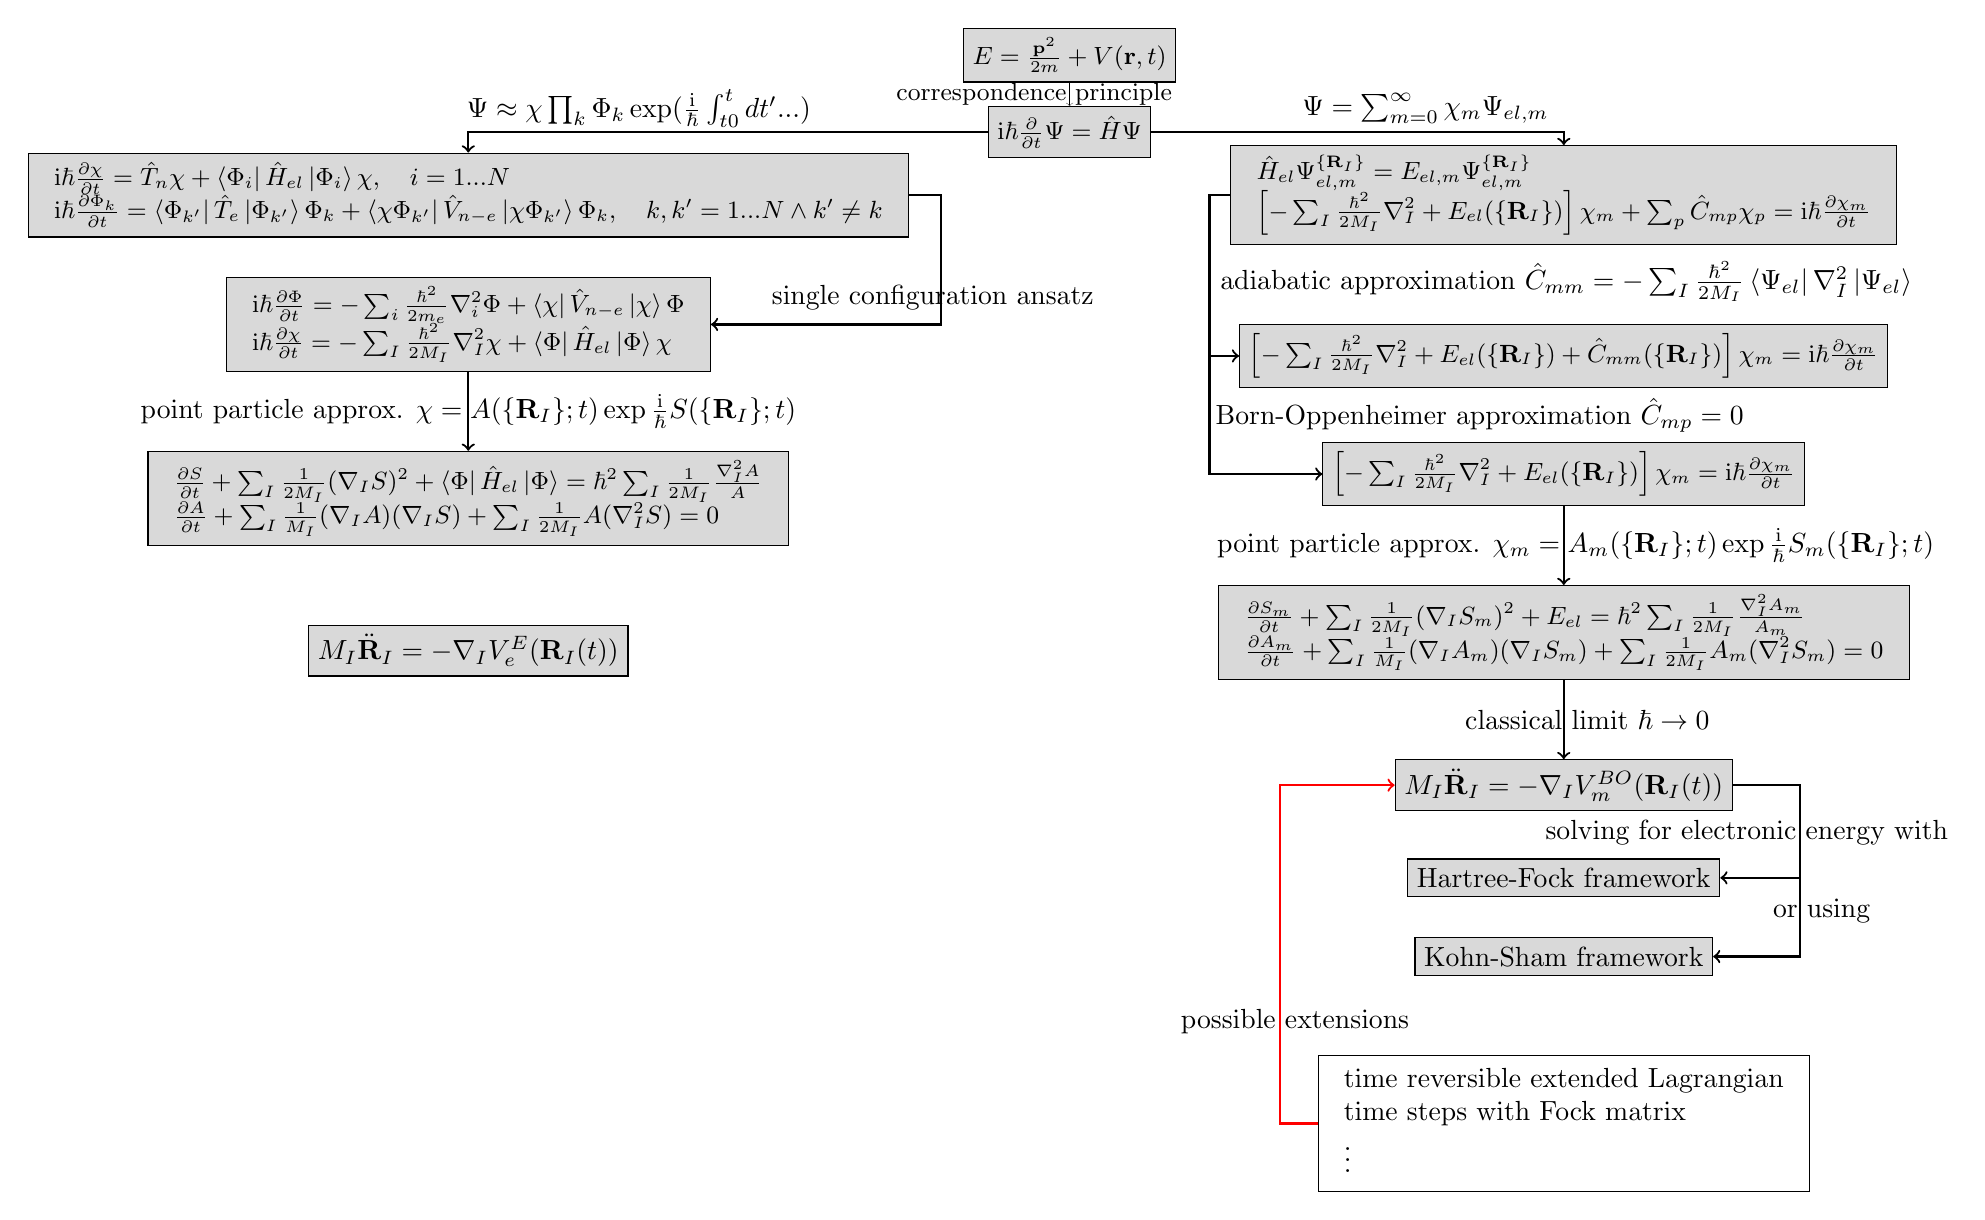
\begin{tikzpicture}[
	  scale=1.0,
	  %style for arrows
	  arrw/.style={thick, ->, >=to},
      % fisrt style for boxes      
      op/.style={rectangle, fill=black!15, draw=black},
      % second style for boxes
      dt/.style={rectangle, fill=white, draw=black}]
            
    % nodes
    \node[op] (root) {\small $E=\frac{\mathbf{p}^2}{2m}+V(\mathbf{r},t)$};
    \node[op, below=3mm of root] (tdse) {\small $\mathrm{i}\hbar\frac{\partial}{\partial t}\Psi=\hat{H}\Psi$};
    %right side
    \node[op, left=of tdse,yshift=-0.8cm] (scfa) 
    {\small \begin{tabular}{l}
	$\mathrm{i}\hbar \frac{\partial \chi}{\partial t} = \hat{T}_n\chi+  \Bra{\Phi_i} \hat{H}_{el}\Ket{\Phi_i} \chi, \quad  i=1...N$\\
$\mathrm{i}\hbar \frac{\partial\Phi_k}{\partial t}= \Bra{\Phi_{k'}} \hat{T}_e\Ket{\Phi_{k'}} \Phi_k + \Bra{\chi\Phi_{k'}} \hat{V}_{n-e} \Ket{\chi\Phi_{k'}} \Phi_k, \quad k,k'=1...N \wedge k'\neq k $\\    
   \end{tabular} }; 
    \node[op, below=of scfa,yshift=0.5cm] (scfsingle){
    \small \begin{tabular}{l}
    $\mathrm{i}\hbar\frac{\partial \Phi}{\partial t}=-\sum_i\frac{\hbar^2}{2m_e}\nabla_i^2\Phi+\Bra{\chi}\hat{V}_{n-e}\Ket{\chi}\Phi$\\ 
    $\mathrm{i}\hbar\frac{\partial \chi}{\partial t}=-\sum_I\frac{\hbar^2}{2M_I}\nabla_I^2\chi+\Bra{\Phi}\hat{H}_{el}\Ket{\Phi}\chi$        	\end{tabular} };
    
    \node[op,below=of scfsingle] (scfsinglepp){
    \small \begin{tabular}{l}
    $\frac{\partial S}{\partial t}+ \sum_I\frac{1}{2M_I}(\nabla_IS)^2+\Bra{\Phi}\hat{H}_{el}\Ket{\Phi}=\hbar^2\sum_I\frac{1}{2M_I}\frac{\nabla_I^2A}{A}$\\
    $\frac{\partial A}{\partial t}+\sum_I\frac{1}{M_I}(\nabla_IA)(\nabla_IS)+\sum_I\frac{1}{2M_I}A(\nabla_I^2S)=0$
    \end{tabular} };
    
    \node[op,below=of scfsinglepp] (ehrenfestmd){$M_I\ddot{\mathbf{R}}_I=-\nabla_IV_e^{E}(\mathbf{R}_I(t))$};
     
     %left side		
     \node[op,right=of tdse,yshift=-0.8cm] (eigenfunc) {\small \begin{tabular}{l}
     $\hat{H}_{el}\Psi_{el,m}^{\{\mathbf{R}_I\}}=E_{el,m}\Psi_{el,m}^{\{\mathbf{R}_I\}}$\\
     $\left[-\sum_I\frac{\hbar^2}{2M_I}\nabla_I^2+E_{el}(\{\mathbf{R}_I\})\right]\chi_m+\sum_p\hat{C}_{mp}\chi_p=\mathrm{i}\hbar\frac{\partial \chi_m}{\partial t}$
     \end{tabular} };
     
     \node[op, below =of eigenfunc,yshift=0cm] (adiabatic) {\small $\left[-\sum_I\frac{\hbar^2}{2M_I}\nabla_I^2+E_{el}(\{\mathbf{R}_I\})+\hat{C}_{mm}(\{\mathbf{R}_I\})\right]\chi_m=\mathrm{i}\hbar\frac{\partial \chi_m}{\partial t}$};
     \node[op, below =of eigenfunc,yshift=-1.5cm] (boapprox) {\small  $\left[-\sum_I\frac{\hbar^2}{2M_I}\nabla_I^2+E_{el}(\{\mathbf{R}_I\})\right]\chi_m=\mathrm{i}\hbar\frac{\partial \chi_m}{\partial t}$};
     
     \node[op, below=of boapprox] (boapprpp){
     \small \begin{tabular}{l}
	$\frac{\partial S_m}{\partial t}+\sum_I\frac{1}{2M_I}(\nabla_IS_m)^2+E_{el}=\hbar^2\sum_I\frac{1}{2M_I}\frac{\nabla_I^2A_m}{A_m}$\\
	$\frac{\partial A_m}{\partial t}+\sum_I\frac{1}{M_I}(\nabla_IA_m)(\nabla_IS_m)+\sum_I\frac{1}{2M_I}A_m(\nabla_I^2S_m)=0$
     \end{tabular} };
     
     \node[op,below=of boapprpp] (bomd) {$M_I\ddot{\mathbf{R}}_I=-\nabla_IV_m^{BO}(\mathbf{R}_I(t))$};
     
     \node[op,below=of bomd,yshift=0.4cm] (hfhamilton){Hartree-Fock framework};
     \node[op,below=of bomd,yshift=-0.6cm] (kshamilton){Kohn-Sham framework};
     
     \node[dt,below=of kshamilton] (boextension) {
     \begin{tabular}{l}
     time reversible extended Lagrangian\\
     time steps with Fock matrix\\
     $\vdots$
     \end{tabular} };
     
    % edges    
    \draw[->,line width=0.1] (root) -- node[xshift=-0.45cm]{\small correspondence principle } (tdse);
    %right side
    \draw[arrw] (tdse) -- node[xshift=1cm,yshift=0.3cm]{$\Psi=\sum_{m=0}^{\infty}\chi_m\Psi_{el,m}$} ++(6,0) -| (eigenfunc);
    \draw[arrw] (eigenfunc) -- node[xshift=4.4cm,yshift=-1.1cm]{adiabatic approximation $\hat{C}_{mm}=-\sum_I\frac{\mathrm{\hbar^2}}{2M_I}\Bra{\Psi_{el}}\nabla_I^2\Ket{\Psi_{el}}$} ++(-4.5,0) -| ++(0,-2.0) |- (adiabatic);
    \draw[arrw] (eigenfunc) -- node[xshift=3.3cm,yshift=-2.8cm]{Born-Oppenheimer approximation $\hat{C}_{mp}=0$} ++(-4.5,0) -| ++(0,-3.5) |- (boapprox);
    \draw[arrw] (boapprox) -- node[xshift=0.15cm]{point particle approx. $\chi_m=A_m(\{\mathbf{R}_I\};t)\exp\frac{\mathrm{i}}{\hbar}S_m(\{\mathbf{R}_I\};t)$} (boapprpp);
    \draw[arrw] (boapprpp) -- node[xshift=0.3cm]{classical limit $\hbar \to 0$} (bomd);
    \draw[arrw] (bomd) -- node[xshift=-0.25cm,yshift=-0.6cm]{solving for electronic energy with} ++(3,0) -| ++(0,-1.20) |- (hfhamilton);
    \draw[arrw] (bomd) -- node[xshift=0.70cm,yshift=-1.6cm]{or using} ++(3,0) -| ++(0,-2.17) |- (kshamilton);
    \draw[arrw,red] (boextension) --node[xshift=-0.05cm,yshift=1.3cm,black]{possible extensions} ++(-3.6,0)-| ++(0,4.0) |- (bomd);
    %left side
    \draw[arrw] (tdse) -- node[xshift=-4.2cm,yshift=0.3cm] {$\Psi \approx \chi \prod_k \Phi_k \exp(\frac{\mathrm{i}}{\hbar}\int_{t0}^{t}dt'...)$} ++(-1.5,0) -| (scfa);
    \draw[arrw] (scfa) -- node[xshift=0.1cm,yshift=-1.3cm]{single configuration ansatz} ++(6,0) -| ++(0,-1.5) |- (scfsingle);
    \draw[arrw] (scfsingle) -- node[xshift=0cm,yshift=0cm]{point particle approx. $\chi=A(\{\mathbf{R}_I\};t)\exp\frac{\mathrm{i}}{\hbar}S(\{\mathbf{R}_I\};t)$} (scfsinglepp);
\end{tikzpicture}
  
\end{document}